\chapter{Introduction}
\label{chap:introduction}

\section{Background for the choice of the topic}
\label{sec:background}

% WHY THIS MATTERS
In 2024, Norway registered 124 fatalities and serious injuries in intersection accidents. This was nearly a 30\% increase compared to the average of the previous four years and the highest level since 2015 \citep{trafikksikkerhetsutviklingen2024}. Intersections are among the most demanding traffic environments, where motor vehicles, cyclists, and pedestrians interact within limited space. This creates numerous potential conflict points. 

In current practice, traffic data at intersections is commonly collected through manual registrations. These are short-term, periodic observations that typically last 1-4 hours and are often limited to peak periods \citep{SVV_V714}. This approach is labor-intensive, and captures only a snapshot of traffic conditions, making it poorly suited for characterizing temporal variation across time of day, weekdays, or seasons.
In current practice, traffic data at intersections is commonly collected through manual registrations. These are short-term, periodic observations that typically last 1–4 hours and are often limited to peak periods \citep{SVV_V714}. This approach is labor-intensive and captures only a snapshot of traffic conditions, making it poorly suited for characterizing temporal variation across time of day, weekdays, or seasons.

Norway has pursued a systematic approach to reduce road traffic fatalities over several decades. Annual deaths have fallen from approximately 500 in the 1970s to 87 in 2024 \citep{trafikksikkerhetsutviklingen2024, regjeringen2024_meldst14}. This progress is closely linked to Vision Zero, anchored in the National Transport Plan (NTP) from 2001. The plan aims to eliminate all road traffic fatalities by 2050, with interim targets for 2030, as shown in \autoref{fig:drept_hardt_skadde} \citep{regjeringen2024_meldst14}. However, recent trends suggest Norway is not on track to meet these targets.

\begin{figure}[H]
    \centering
    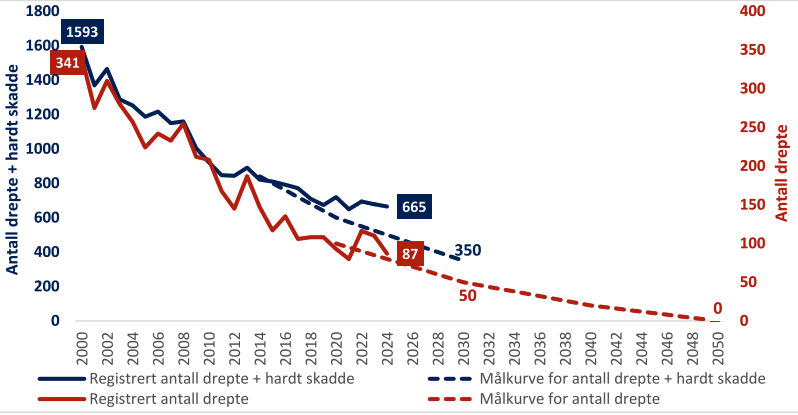
\includegraphics[width=0.9\linewidth]{project/images/fatalitiesandinjured.png}
    \caption[Development in road traffic fatalities and serious injuries in Norway]{Development in road traffic fatalities and serious injuries in Norway, with interim targets for 2030 and 2050 \citep{trafikksikkerhetsutviklingen2024}}.
    \label{fig:drept_hardt_skadde}
\end{figure}

Intersections account for a disproportionate share of road traffic casualties. Despite the overall reduction in fatalities and serious injuries since 2001, their share has not declined correspondingly~\citep{svv_trine}. This indicates a continued need for targeted safety measures at these locations, as illustrated in \autoref{fig:prosentandel_kryss}.

\begin{figure}[H]
    \centering
     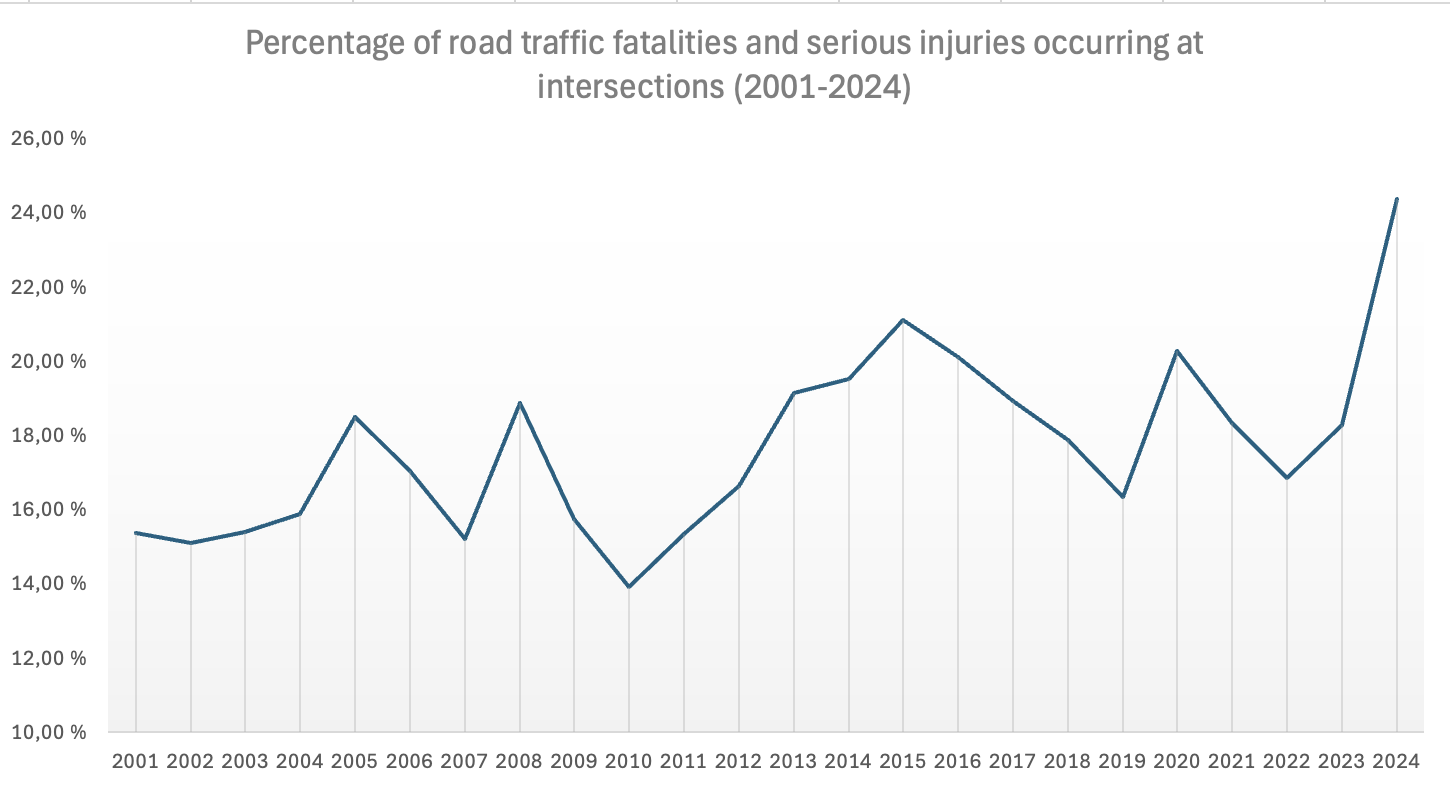
\includegraphics[width=0.8\linewidth]{project/images/prosentandel_kryss.png}
    \caption[Percentage of road traffic fatalities and serious injuries occurring at intersections (2001-2024)]
    {Percentage of road traffic fatalities and serious injuries occurring at intersections (2001-2024). Based on data from TRINE \citep{svv_trine}.}
    \label{fig:prosentandel_kryss}
\end{figure}

Norway's long-term transport policy is outlined in the NTP 2025–2036 \citep{regjeringen2024_meldst14}. It emphasizes that digital solutions, new technology, and artificial intelligence can fundamentally change how people and goods are transported. The plan links these tools to improved efficiency and core policy goals such as Vision Zero and reduced environmental impact. In traffic management specifically, it notes that AI can analyze large traffic data streams. It can predict flow and congestion patterns, enabling real-time adjustments of traffic signals, lane usage, and roadside signage.

A central motivation for this thesis is the NTP's explicit recognition that fiscal constraints are tightening. Rising costs in ongoing projects and tighter public budgets are reducing the financial room for new infrastructure investments \citep{regjeringen2024_meldst14}. The plan responds by shifting emphasis toward maintenance, renewal, and solutions that extract greater value from existing assets. This makes a compelling case for examining whether infrastructure already in place, such as fixed roadside cameras, can serve as reliable data sources for traffic monitoring. If existing video installations can be analyzed with AI-based methods, traffic monitoring and safety assessments can be expanded. This, at substantially lower marginal costs than approaches requiring new sensor deployments or repeated manual registrations. Several local authorities abroad are already applying AI to CCTV and video sensors for automated traffic and pedestrian monitoring \citep{ITSKRSComputerVisionCCTV, VivacityValidation2022}.

%What remains unresolved is whether these methods perform reliably enough under real operating conditions to support traffic management decisions. Factors such as variable lighting, weather, occlusion, and camera placement remain insufficiently tested. Existing validation studies are typically conducted under controlled or near-ideal conditions, leaving a gap between reported accuracy and operational deployability. The following section maps this gap in detail and identifies the specific questions this thesis addresses.

\section{Knowledge Gap}
Computer vision (CV) has become an increasingly important component of intelligent transportation systems (ITS). Comprehensive survey studies show that vision-based methods are applied across a wide range of transportation tasks and play a growing role in improving traffic monitoring, safety, and operational efficiency \citep{CVSurvey}.

Previous studies demonstrate that deep learning–based object detection models, particularly YOLO-based architectures, can achieve high accuracy and near real-time performance for vehicle detection and counting. This has been shown in established benchmark datasets and in constrained traffic environments \citep{Everingham10,HuggingFacePascalVOC, Song2019VisionBasedVehicle, smartcities6050134, YOLO-PEL}.

However, the literature also identifies limitations that motivate the research questions in this thesis. \citet{Maity2022LastDecadeVehicleDetection} highlights that many Automatic Vehicle Detection (AVD) studies rely on a limited set of vehicle classes. This motivates \textbf{Research Question 1} on detailed vehicle classification. The same survey further notes that robustness is often not explicitly evaluated under occlusion and dense traffic. Together with reported challenges in adverse lighting and weather, and in small-object/multi-scale detection \citep{DeepLearningTrafficScene2025,YOLO-PEL}, this motivates \textbf{Research Question 2} on performance under varying operational conditions. Finally, calls for practical validation in real-world deployments \citep{YOLO-PEL} and the need for more robust, end-to-end tracking pipelines for complex scenarios \citep{Hassan2024} motivate \textbf{Research Question 3}. This question concerns sustained autonomous operation and reliability over time.


\section{Problem Statement and Research Questions}
\label{sec:rq}

Building on the knowledge gap identified in the previous section, this thesis evaluates how deep learning-based detection and tracking systems can be configured to extract accurate traffic parameters from intersection video. The focus is on detailed vehicle classification and turning movement counts. Existing systems are typically validated on limited vehicle classes and over short evaluation periods. This leaves open questions about performance under varying conditions and sustained autonomous operation during dynamic lighting transitions. The three research questions address these gaps and maintain a clear thread from the literature review to the problem statement.

  
    \textbf{RQ1: How accurately can deep learning-based detection models extract detailed vehicle classification at an intersection?} 
    
    \textbf{RQ2: How do different model configurations (detector + tracker) perform in extracting turning movement counts under varying lighting conditions?}
    
    \textbf{RQ3: To what extent can a vision-based traffic monitoring system operate autonomously over time without manual intervention?}


%Can an adaptive dual-tracker system that automatically switches between optimized day- and nighttime configurations maintain reliable turning movement extraction across lighting transitions without manual intervention?


\section{Scope and limitations}
% WHAT WE WON´T COVER

\subsection*{Scope}
This study is delimited as follows:
\begin{itemize}
    \item \textbf{Geographic:} Analysis of one T-intersection in Norway.

    \item \textbf{Model scope:} Evaluation of YOLO26, the most recent YOLO release, specialized on traffic object detection.

    \item \textbf{Parameters:} Focus on traffic volumes, vehicle composition, turning movements, and the presence of pedestrians.
    
   \item \textbf{Temporal:} Video data collected during February-April 2026, capturing variations across the time of day and weather conditions.
    
\end{itemize}

\subsection*{Limitations}

The study has the following limitations:

\begin{itemize}

    \item \textbf{Camera and privacy constraints:} The traffic camera was not positioned or configured for optimal object detection. Certain areas of the video are intentionally blurred to comply with the General Data Protection Regulation (GDPR) requirements. This may affect detection performance near privacy-masked regions. 
    
    
    \item \textbf{Environmental conditions:} Detection performance may be affected by weather (rain, snow, fog) and lighting conditions (night, shadows).

    \item \textbf{Intersection type:} The pipeline is limited to a T-intersection. Findings may not generalize, as different geometries or camera configurations are unknown.


    \item \textbf{Vulnerable road users:} Low instance counts of cyclists and pedestrians in the dataset limit the reliability of performance estimates for these classes.
    
    
\end{itemize}


\section{Structure of The Thesis}
% HOW THE THESIS IS ORGANIZED~
The thesis is structured as follows: Chapter~\ref{chap:theory} reviews existing traffic registration methods, object detection theory, and relevant literature on YOLO architectures and multi-object tracking. Chapter~\ref{chap:methods} describes the dataset development and the fine-tuning of YOLO26 models for detailed classification. It also presents the implementation of a dual-configuration tracking pipeline using BoT-SORT and ByteTrack. Chapter~\ref{chap:results} presents detection and tracking performance across varying lighting conditions. Chapter~\ref{chap:discussion} discusses the results and addresses the research questions in relation to prior work. Chapter~\ref{chap:conclusion} summarizes the contributions and directions for future research. Supplementary material, including implementation code and raw results, is provided in the appendices.
